\chapter{Project}
%\label{chapter:title}
\section{The context}

The idea of processing in memory is an old one and has been considered since the mid 1990s~\cite{stone1970logic, Kautz1969, shaw1981non, kogge1994, gokhale1995processing, patterson1997case, oskin1998active, kang1999flexram, Mai:2000:SMM:339647.339673, Draper:2002:ADP:514191.514197,aga.hpca17,eckert2018neural,fujiki2019duality,kang.icassp14,seshadri.micro17,seshadri2013rowclone,angizi2019graphide,kim.hpca18,kim.hpca19,gao2020computedram,chang.hpca16,xin2020elp2im,li.micro17,deng.dac2018,hajinazarsimdram,rezaei2020nom,wang2020figaro,ali2019memory,li.dac16,angizi2018pima,angizi2018cmp,angizi2019dna,levy.microelec14,kvatinsky.tcasii14,shafiee2016isaac,kvatinsky.iccd11,kvatinsky.tvlsi14,gaillardon2016plim,bhattacharjee2017revamp,hamdioui2015memristor,xie2015fast,hamdioui2017myth,yu2018memristive,syncron,fernandez2020natsa,cali2020genasm,kim.bmc18,ahn.pei.isca15,ahn.tesseract.isca15,boroumand.asplos18,boroumand2019conda,singh2019napel,asghari-moghaddam.micro16,DBLP:conf/sigmod/BabarinsaI15,chi2016prime,farmahini2015nda,gao.pact15,DBLP:conf/hpca/GaoK16,gu.isca16,guo2014wondp,hashemi.isca16,cont-runahead,hsieh.isca16,kim.isca16,kim.sc17,DBLP:conf/IEEEpact/LeeSK15,liu-spaa17,morad.taco15,nai2017graphpim,pattnaik.pact16,pugsley2014ndc,zhang.hpdc14,zhu2013accelerating,DBLP:conf/isca/AkinFH15,gao2017tetris,drumond2017mondrian,dai2018graphh,zhang2018graphp,huang2020heterogeneous,zhuo2019graphq,santos2017operand,ghoseibm2019,wen2017rebooting,besta2021sisa,ferreira2021pluto,olgun2021quactrng,lloyd2015memory,elliott1999computational,zheng2016tcam,landgraf2021combining,rodrigues2016scattergather,lloyd2018dse,lloyd2017keyvalue,gokhale2015rearr,nair2015active,jacob2016compiling,sura2015data,nair2015evolution,balasubramonian2014near,xi2020memory}.
Despite being the first company to reach the stage of a commercially available PIM product, UPMEM is in need of more technological demonstrators to encourage widespread adoption of its system.

My role during this apprenticeship was to develop machine-learning applications running on PIM that display an enticing performance gain (be it speed or energy consumption) when compared to existing CPU or GPU implementations.

\subsection{The technology}

\subsubsection{Motivation}

Data transfer on SDRAM is limited by a communication bus. Currently, the transfer rate on DDR5-6400 is 51.2 GB/s per channel (409.6 GB/s on an 8-channel system). Although this speed has been steadily increasing, there are popular algorithms today that end up with memory-bound performances (such as pooling operations in neural networks~\cite{nvidia.memory2020}).

The principle of PIM is to execute as many operations as possible in memory, and to minimize the number of operations that are executed in the CPU, thus limiting the flow of data through the memory bus.

\subsubsection{Architecture}

UPMEM DIMM is based on DDR4 and attaches an onboard RISC-V processor to each 64 MB memory bank, these processors are called DPU for Data Processing Units. A schematic representation of an UPMEM DIMM can be seen in Figure \ref{fig:DIMM}. The DPUs access their MRAM via a DMA engine. The transfer rate between each DPU and its associated memory bank (called MRAM) is 1 GB/s. This means that on a server with the maximum number of DPUs (2560), the total transfer rate is 2.5 TB/s. Each DPU can execute up to 24 tasklets in parallel.

\begin{figure}[htb]
    \centering
    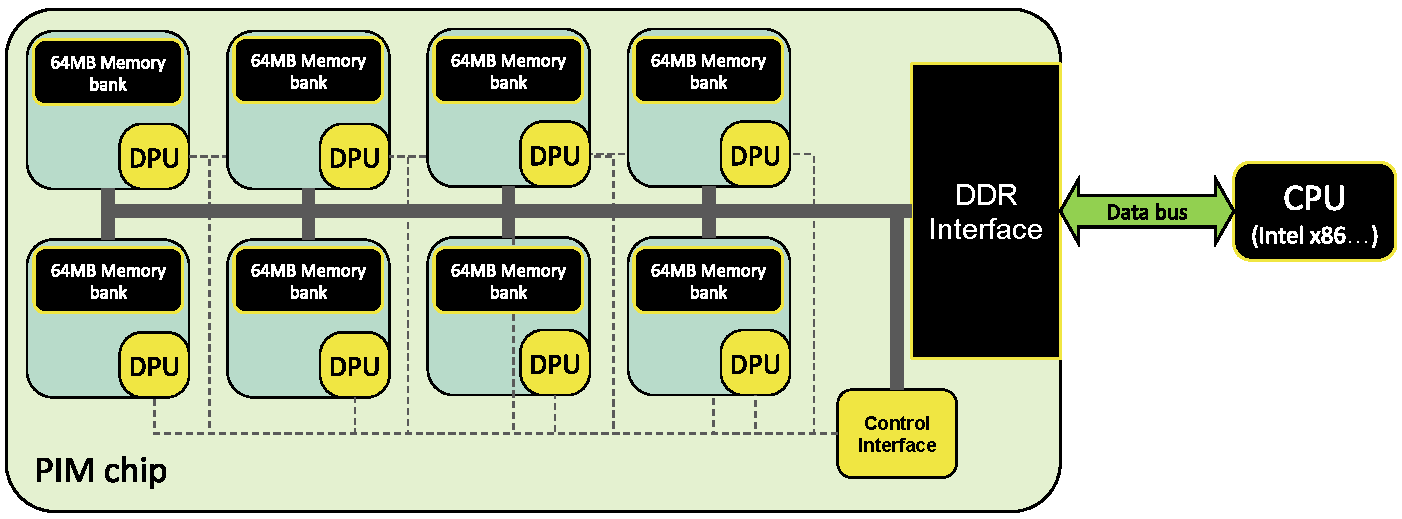
\includegraphics[width=0.95\linewidth]{figures/PIM.pdf}
    \caption{\label{fig:DIMM}UPMEM PIM Architecture}
\end{figure}

Each DIMM has two ranks with 64 DPUs each. This amounts to 8.2 GB of memory per DIMM. Each DPU also has an internal Work RAM (WRAM) of 64 KB.

In reality, at the hardware level, DPUs come in pairs, and each pair is connected to a memory bank. However, this is entirely transparent to the programmer. Therefore, we will ignore this fact.

\subsubsection{Limitations}
\label{subsubsection:Limitations}

A number of engineering choices had to be made to make UPMEM PIM a viable product. We will now list the ones that are most relevant to developers:

\begin{itemize}
    \item \textbf{Floating point arithmetic:} Due to the limited space available on the chip, the DPUs do not have a floating point unit, and therefore do not support floating point operations at the hardware level. It is still possible to perform floating point operations on the DPUs, but these are simulated operations, and therefore much slower than hardware supported operations. For example, a single 32-bit floating point operation on a DPU will take upwards of 120 instructions.
    \item \textbf{Discrete arithmetic:} At the hardware level, the DPUs support 32 bits integer additions/subtractions, and 8 bits integer multiplications.
    \item \textbf{Parallelism:} Being RISC processors, the DPUs need to execute instructions in parallel to take full advantage of the available resources. Instructions in a DPU go through a pipeline of 11 stages when they execute. Thus, we need to use at least 11 tasklets to reach peak performance. In practice, we generally use 16 tasklets because it's a power of two, and because the extra tasklets can sometimes hide the latency of DMA accesses. Tasklets can synchronize via mutexes or semaphores, but this has a performance cost and should be kept to a minimum.
    \item \textbf{Stack size:} Each DPU has to share its WRAM between its tasklets, and generally keep some space for global variables. This usually leaves 1 KB or 2 KB of stack for each tasklet.
    \item \textbf{DMA memory accesses:} Accessing the MRAM is slower than the WRAM, and it incurs some overhead. Therefore, MRAM accesses should be done in large blocks, or streamed with a sequential reader. Performing too many random accesses impacts performance negatively. Also, there are alignment constraints: each memory access has to be aligned on 8 bytes. Forgetting that fact can lead to concurrency issues if two tasklets try to modify two values in the same 8-byte aligned memory location.
    \item \textbf{Compilation:} The DPU kernels are compiled with a modified version of the LLVM compiler. While it does generally perform as expected, the C standard was mostly created with x86 processors in mind. This means that sometimes the compiler will generate code that is not optimized for the target architecture. An example of that behavior can be seen in section %\ref{sec:compilation}.
\end{itemize}